\section{Архитектура и модули системы}

Разработанное программное средство состоит из следующих модулей:
\begin{itemize}
    \item модуль выделения признаков почерка;
    \item модуль определения параметров личности;
    \item модуль контроля доступа;
    \item модуль доступа к базе данных.
\end{itemize}

Вышеописанные модули опираются на следующие группы классов, разработанные в рамках дипломного проекта:
\begin{itemize}
    \item Набор классов для сегментации изображения на строки, слова, символы и выделения признаков. Написан на языке Scala с использование сторонней библиотеки OpenCV.
    \item Набор классов машинного обучения (для классификации признаков текста). Написан на языке программирования Scala и содержит реализацию алгоритма основанного на методе опорных векторов (Support Vector Machine), о котором будет рассказано далее.
    \item Набор классов для контроля доступа. Написана на языке Scala. Содержит классы для регистрации, авторицации и управлением сессией пользователя. Основан на стандарте JSON Web Token (JWT).
    \item Набор классов для организации храниения и доступа в авторизационным данным пользователя и коллекции обработанных изображений.
\end{itemize}

Далее будет подробно описана структура и назначения каждого модуля.

\afterpage{
  \begin{landscape}
  \thispagestyle{lscape}
  \begin{figure}[t!]
  \centering
    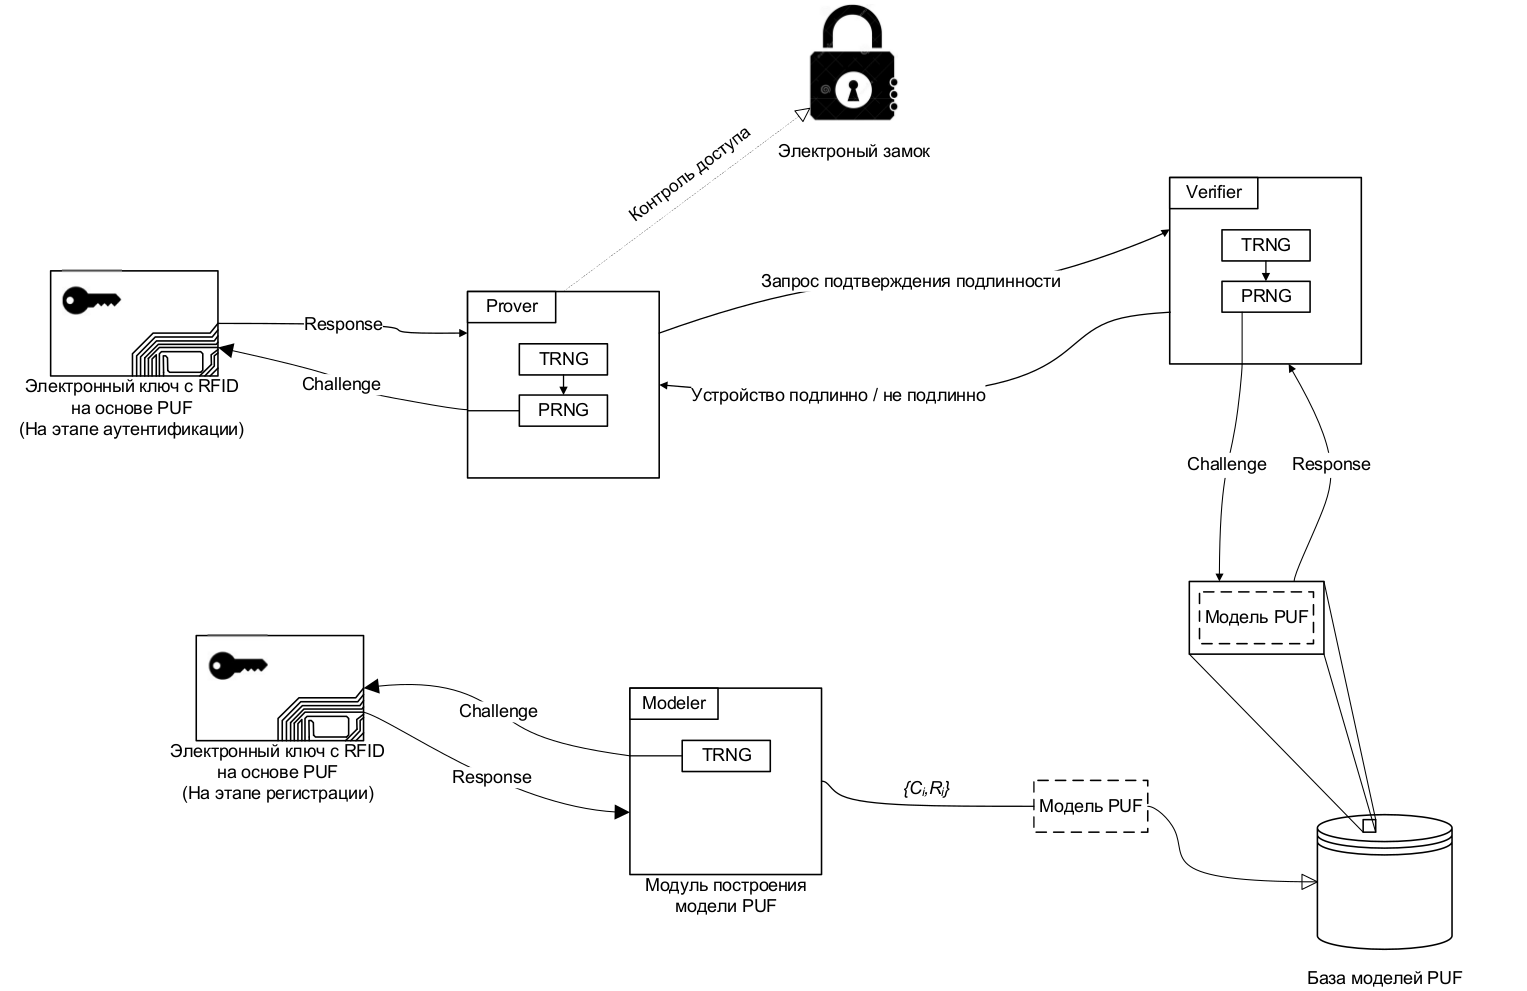
\includegraphics[scale=0.40]{figures/flow.png}
    \caption{ Схема работы программной системы }
    \label{fig:architecture:flow}
  \end{figure}
  \end{landscape}
}

\subsection{Модуль определения параметров личности}

Для определения параметров личности по признаком рукописного текста был выбран классификатор на основе метода опорных векторов -- широко используемый метод машинного обучения~\cite{manning_ir}, который при своей относительной простоте реализации, позволяет добиться очень неплохих результатов классификации.

Метод опорных векторов (\emph{SVM, support vector machine}) – семейство схожих алгоритмов обучения с учителем, использующихся для задач классификации и регрессионного анализа. Особым свойством метода опорных векторов является непрерывное уменьшение эмпирической ошибки классификации и увеличение зазора, поэтому метод также известен как метод классификатора с максимальным зазором.~\cite{mitchell_ml, wiki_SVM}:

Параметры текста представляют собой непрерывные величины подчиняющиеся нормальному распределению, исходя из этого в качестве ядер используются радиально-базисная функция Гаусса~\cite{gauss_wiki}.

\begin{equation}
  \label{eq:architecture:gaussian_core}
  k(x, x^{'}) = \exp(-\frac{\left|\left| x - x^{'} \right|\right|}{2\sigma_{}^2})
\end{equation}
\begin{explanation}
где & $x^{'}$ & среднее значение параметра, рассчитанное для объектов, принадлежащих
классу $C$; \\
    & $ \sigma_{}^2 $ & дисперсия значания параметра объектов из класс $C$.
\end{explanation}

Дисперсия значения параметра:
\begin{equation}
  \label{eq:architecture:dispersion}
  \sigma_{}^2 = \frac{1}{n - 1} \sum\limits_{x \in C} (x_i - \overline{x_{}}^2)
\end{equation}

\begin{figure}[!h]
    \centering
    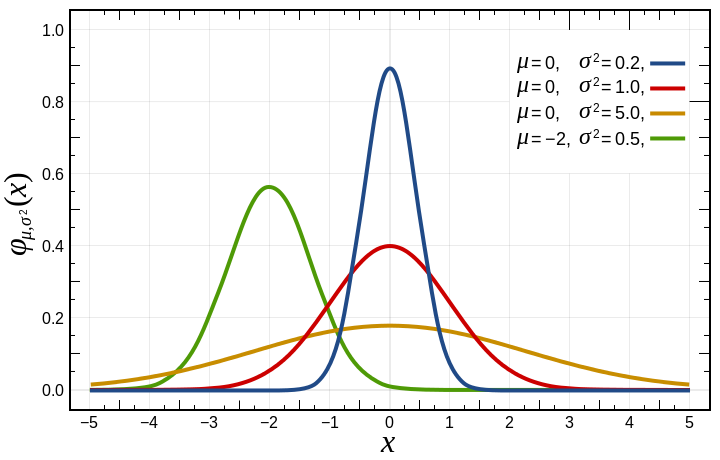
\includegraphics[width=0.85\textwidth]{figures/gauss.png}
    \caption{График функции плотности вероятности для нормального распределения}
    \label{fig:architecture:normal_pd}
\end{figure}

\subsection{Модуль выделения признаков почерка}
Основным функциями данного модуля является:
\begin{itemize}
  \item подготовка изображения к обработке (бинаризация, удаление шумов);
  \item сегментация текста (строки, слова, символы);
  \item выделения признаков подчерка.
\end{itemize}

На это этапе обработки используется алгоритм линейной бинаризации по пороговому значению доминантного цвета, посколько обработке подверкается образцы почерка с высокой вероятностью это будет цвет чернил.
Математическое выражение линейной бинаризации выглядит следующим образов:

\begin{equation}
  \label{eq:architecture:liner_binarisation}
 \left \{
  \begin{tabular}{l}
   x <  T, x = 0 \\
   x $ \geq $ T, x = 255
  \end{tabular}
   \right .
\end{equation}
\begin{explanation}
где & $ x $ & значения яркости цвета пикселя; \\
    & Т & порог бинаризации.
\end{explanation}

Для удаления шумов используется фильтр максимума - минимума. Алгоритм работы данного фильтра основан на замене текущего пикселя на пиксель с максимальной яркостью из его окресности при первом проходе и на пиксель с минимальной при повторном. Данный алгоритм хорошо справляется с импульсными шумами и шумами типа <<соль и перец>>.

Следующий этапам является сегментация изображения, а первой стадией сегментации является сегментация строк. 
Задача выделения строк сводиться к нахождению верхних и нижних граней строк текста на исходном изображении. Алгоритм сегментации строк основывается на том, что средняя яркость в изображениях межстрочных промежутках существенно ниже средней яркости в изображениях текстовых строк~\cite{cv_text_image_segmentator}.

Первым этапом необходимо для всех пиксельных строк исходного изображения находим их средние значения яркости
\begin{displaymath}s_j = s_j(B) = \frac{1}{n}\cdot\sum\limits_{i=1}^{n} b_{ij}\end{displaymath}

Затем определяем среднее значение яркости всего изображения
\begin{displaymath}s(B) = \frac{1}{m}\cdot\sum\limits_{j=1}^{m} s_j(B)\end{displaymath}

Средняя яркость в межстрочных промежутках текста должна быть невелика (в идеальном случае она равна нулю). Поэтому яркость верхней границы текстовой строки можно выразить через среднюю яркость изображения
\begin{displaymath}s^{t} = k^{t} * s(B)\end{displaymath}

где 0<kt<1 - коэффициент

Аналогично яркость нижней границы текстовой строки, также может быть выражена через среднюю яркость всего изображения
sb= kb * s(B)

где 0<kb<1 - коэффициент

Работа алгоритма сегментации строк заключается в последовательном просмотре массива средних значений (s1,...,sm) и выявлении множества пар индексов (sti,sbi) пиксельных строк, соответствующих верхней sti и нижней sbi граням изображения строки номер i, удовлетворяющих следующим условиям.

Условия верхней границы текстовой строки:
\begin{itemize}
  \item яркость текущей пиксельной строки превышает границу $ s^{t} $
  \item яркость двух предыдущих пиксельных строк ниже этой границы
  \item яркость трех последующих строк выше границы $ s^{b} $
\end{itemize}

Следовательно должно выполняться логическое условие:
\begin{displaymath}(s_{i-2} < s^{t}) \wedge (s_{i-1} < s^{t}) \wedge (s_i > s^{b}) \wedge (s_{i+1} > s^{b}) \wedge (s_{i+2} > s^{b}) \wedge (s_{i+3} > s^{b})\end{displaymath}

Условия нижней границы текстовой строки.
\begin{itemize}     
  \item было зафиксировано начало области
  \item яркость текущей пиксельной строки превышает границу $ s^{t} $
  \item яркость последующей пиксельной строки ниже границы $ s^{b} $
\end{itemize}
     
или

\begin{itemize}
   \item было зафиксировано начало области
   \item яркость трех последующих строк ниже границы $ s^{b} $
\end{itemize}

Следовательно должно выполняться логическое условие:
\begin{displaymath}((s_{i+1} < s^{b}) \wedge (s_{i+2} < s^{b}) \wedge (s_{i+3} < s^{b}) \vee ((s_i > s^{t}) \wedge (s_{i+1} < s^{b})))\end{displaymath}

В результате формируется множество пар индексов верхних и нижних граней строк. Разность между этими индексами дает высоты текстовых строк. Однако такой алгоритм находит среднюю высоту каждой текстовой строки и "срезает" символы, выступающие по высоте за эту среднюю высоту.

Чтобы избежать этого, необходимо расширить найденные границы. Можно предложить следующий алгоритм расширения границ. Среди найденных текстовых строк определяется строка с минимальной высотой Hmin и, затем все границы с каждой стороны расширяются на величину 0.3 * Hmin. Это не приводит к слиянию строк, т.к. межстрочные интервалы текста, как правило, больше чем высота строки.
 
Таким образом, в результате работы алгоритма на исходном изображении отмечается положение всех текстовых строк.  

Алгоритмы сегментации слов и символом сходи с алгоритмом сегментации строк. Основными отличиями являются необходимость построения карты яркости столбцов, а не строк, а так наличие дополнительных этапов обработки. Такими этапоми являются приминение <<размазывающего>> фильтра при сегментации слов и удаление ложных границ после сегментации символов. 

Следующей функцией данного модуля является выделение из изображения признаков текста:
\begin{itemize}
  \item наклон символов;
  \item наклон строк;
  \item интервал между символами;
  \item интервал между строками;
  \item частота текста;
  \item сила нажима.
\end{itemize}

Для опреления угла наклона символа необходимо определить координаты верхней и нижней точек символа и используя арктангенс вычислить угол. Мателатичекое выражение:

\begin{equation}
  \label{eq:architecture:symbol_angle}
  \Theta = \tan^{-1}{\frac{y_2 - y_1}{x_2 - x_1}}
\end{equation}
\begin{explanation}
где & $\Theta$ & угол наклона символа \\
    & $ (y_1, y_2) (x_1, x_2) $ & координаты крайних точек сисвола.
\end{explanation}

\begin{figure}[ht]
    \centering
    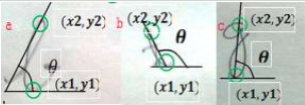
\includegraphics[width=0.85\textwidth]{figures/char_angle.png}
    \caption{Пример рассчета угла между символами}
    \label{fig:architecture:symbol_angle}
\end{figure}

\subsection{Модуль контроля доступа}
Данный модуль отвечает за регистрацию и авторизацию пользователей. Посколько разрабатываемое приложение может содержать персональные данные пользователя, вплодь до имени и фамилии в графе комментариев к изображению, задача организации безопасного доступа и хранению подобных данных стоит довольно остро. 
В данном проекте для предоставления защищенного доступа к модулям будет использоваться открытый стандарт JSON Web Token (RFC 7519). JWT маркер, содержит в зашифрованном виде всю минимально необходимую информацию для аутентификации и авторизации. При этом не требуется хранить в сессии данных о пользователе, так как маркер самодостаточный. Данный факт упрощает горизонтальное масштабирование системы и хорошо подход для архитектур на основе микросервисов.

Основными функциями данного модуля являются:
\begin{itemize}
  \item регистрации новых пользователей;
  \item авторицация пользователей;
  \item генерация JWT маркеров.
\end{itemize}

Обобщеный алгоритм генерации и верификации JWT токенов:
\begin{figure}[ht]
    \centering
    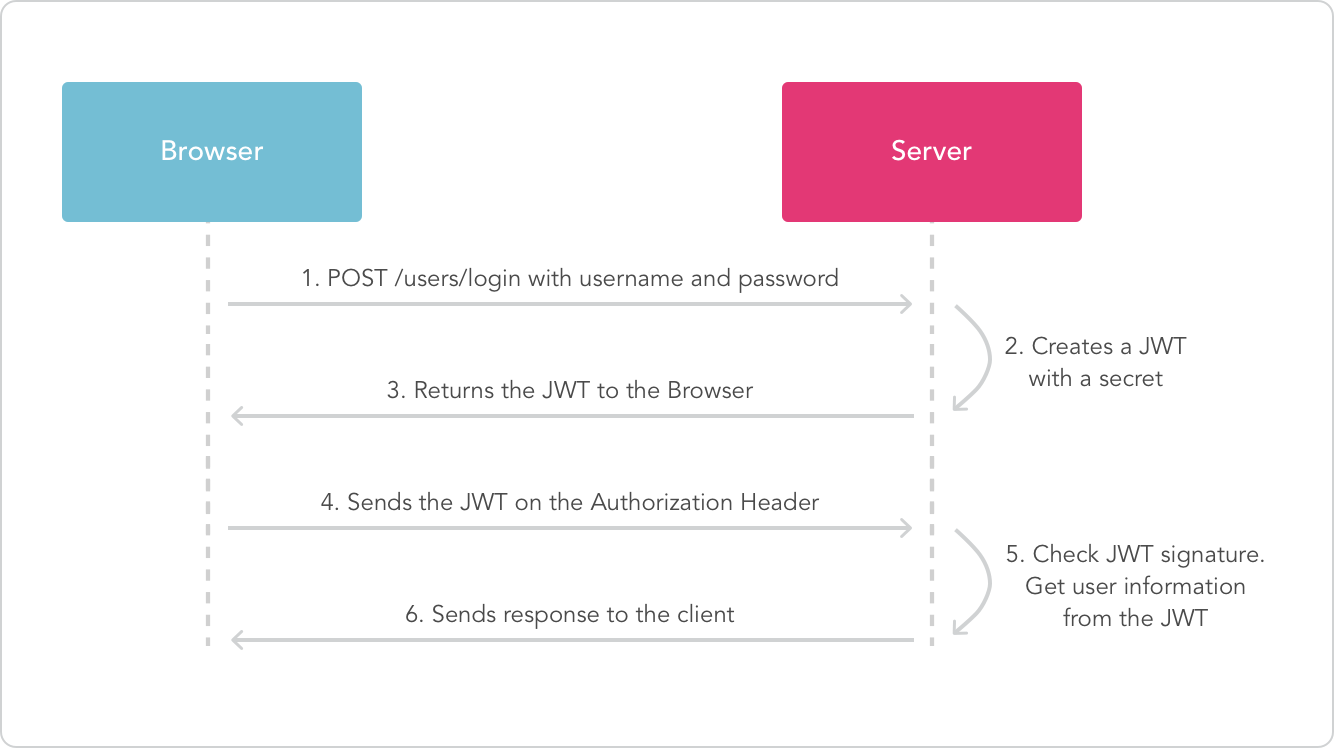
\includegraphics[width=0.7\textwidth]{figures/jwt_diagram.png}
    \label{fig:architecture:jwt_diagram}
    \caption{Диаграмма работы JWT маркетов}
\end{figure}

\subsection{Модуль доступа к данным}
Данный модуль отвечает за организацию работы в базой данных и предоставление другим модулям удобного интерфейса.
Основными функциями данного модуля являются:
\begin{itemize}
  \item добавление авторизационыых данных пользователя в базу при регистрации (включая проверку дублирования имен пользователей);
  \item проверка наличия пользователя в базе и соответвие хеша пароля;
  \item добавление нового изображения в базу;
  \item обновление информации о параметрах изображения;
  \item удаление изображения из базы.
\end{itemize}

NoSQL база данных. Так как список параметров изображения не поспоянный и параметры рассчитываются и обновляются паралельно, использование классической реляционной базы данных в данном случае нерационально. В рамках разработки программное средство используется нереляционной СУБД MongoDB. Так же плюсом является то, что данные храняться в баззе ввиде JSON-объектов, что исключает дополнительное предбразование данных перед отправкой их на клиент.

